\documentclass{article}

\title{CS 579 Project: Extension Complexity of Polytopes in Combinatorial Optimization}
\author{Vasilis Livanos, Manuel Torres \\ Net IDs: livanos3, manuelt2}
\date{May 2, 2018}

\usepackage{amsmath, amssymb}  
\usepackage{fullpage}  
\usepackage{amsthm}  
\usepackage{mathtools}  
\usepackage{complexity}
\usepackage{xspace}

\newtheorem{theorem}{\sc Theorem}
\newtheorem{lemma}[theorem]{\sc Lemma}
\newtheorem{prop}[theorem]{\sc Proposition}
\newtheorem{corollary}[theorem]{\sc Corollary}
\newtheorem{fact}[theorem]{\sc Fact}
\newtheorem{probstate}[theorem]{\sc Problem Statement}
\theoremstyle{definition}
\newtheorem{definition}[theorem]{Definition}
\newtheorem{example}[theorem]{Example}
\theoremstyle{remark}
\newtheorem{remark}[theorem]{\sc Remark}
\newtheorem{claim}[theorem]{\sc Claim}
\newtheorem{observation}[theorem]{\sc Observation}
\newenvironment{proofsketch}{%
  \renewcommand{\proofname}{Proof Sketch}\proof}{\endproof}

\usepackage{hyperref}  % used to hyperlink citations to bibliography
\hypersetup{
    colorlinks=true,
    linkcolor=[rgb]{0,0,0.6},
    citecolor=[rgb]{0,0,0.6}
} % changes color of hyperlinks to help notify the reader of the hyperlinks

\newcommand{\cetal}{\textit{et al.\@}}  % shortcut for etal to be used when no space is desired
\newcommand{\etal}{\textit{et al.\@\ }}  % shortcut for etal to be used in regular text
\newcommand{\nrank}{\operatorname{rank}_+}
\newcommand{\rank}{\operatorname{rank}}
\newcommand{\diag}{\operatorname{diag}}
\newcommand{\bits}{\{0,1\}}
\newcommand{\abs}[1]{\left|#1\right|}
\newcommand{\conv}{\operatorname{conv}}
\newcommand{\suppmat}{\operatorname{suppmat}}
\newcommand{\supp}{\operatorname{supp}}
\newcommand{\ol}[1]{\overline{#1}}
\newcommand{\ul}[1]{\underline{#1}}
\newcommand{\oul}[1]{\overline{\underline{#1}}}
\newcommand{\xc}{\operatorname{xc}}
\newcommand{\TSP}{\operatorname{TSP}}
\newcommand{\STAB}{\operatorname{STAB}}
\newcommand{\CUT}{\operatorname{CUT}}
\newcommand{\COR}{\operatorname{COR}}
\renewcommand{\R}{\mathbb{R}}
\def\problem#1{\textsc{#1}}
\def\HAMPATH{\problem{HAMPATH}\xspace}
\def\THREESAT{\problem{$3$SAT}\xspace}

\newcommand{\vnote}[1]{{\color{magenta}\noindent\textbf{V: }\marginpar{****}\textit{{#1}}}}
\newcommand{\mnote}[1]{{\color{blue}\noindent\textbf{M: }\marginpar{****}\textit{{#1}}}}

\begin{document}
\maketitle

\section{Introduction}

Assuming $\P \ne \NP$, any linear program (LP) for the traveling salesperson problem (\lang{TSP}) must be of super-polynomial size, otherwise one could use the ellipsoid method or interior point method to solve a polynomial-size LP for $\lang{TSP}$ in polynomial time, refuting $\P \ne \NP$. It is also interesting to consider the converse of this statement: if there exists a polynomial-size LP for $\lang{TSP}$, then $\P = \NP$ as $\lang{TSP}$ is $\NP$-complete. This motivates the following question: can we write a polynomial size LP for $\lang{TSP}$? The work of Fiorini~\cetal~\cite{fiorini} attempts to resolve this question and their work is the subject of this exposition.

\subsection{Problem Statement}

The problem is simply stated: find super-polynomial lower bounds for the size of any LP for $\lang{TSP}$. This seemingly daunting task motivates the following definition. 

\begin{definition}[Extended Formulation]
Let $b,d$ be column vectors and let $A$, $B$, and $C$ be real matrices with $n$, $n$, and $r$ columns, respectively. Let $P = \{x \in \R^n : Ax \le b\}$ and $Q = \{(x,y) \in \R^n \times \R^r : Bx + Cy \le d\}$. We say that $Q$ is an \emph{extended formulation} (EF) of $P$ if $P = \{x : \exists y \in \R^r, (x,y) \in Q\}$. The size of $Q$, the EF of $P$, is the number of entries in $d$. That is, the size of the EF $Q$ is the number of inequalities defining $Q$. The \emph{extension complexity} of $P$, denoted by $\xc(P)$, is the minimum size EF of $P$.
\end{definition}

At a basic level, an EF of a polytope $P$ is a polytope $Q$ in a higher-dimensional space with a different set of constraints, but is in essence equivalent to $P$. It is equivalent in the sense that one can optimize over an EF $Q$ of $P$ to optimize over $P$. However, we gain nothing if $Q$ is more complex than $P$. Suppose, for instance, that $P$ is a polytope with $n$ variables and an exponential number of constraints. If there exists an EF $Q$ of $P$ with a polynomial number of variables and constraints in $n$, then it would be possible to optimize over $Q$ in polynomial time as a way of optimizing over $P$. It is not immediately evident that there should even be EFs that can save an exponential number of constraints at the expense of increasing the number of variables polynomially. We give an example in Section~(\ref{sec:utility-EF}) that shows the existence of such an EF.

The notion of an EF gives a direction towards answering the question posed at the beginning of this section. In particular, if one could show that the extension complexity of the $\lang{TSP}$ polytope is exponential, then there would not exist a polynomial-size LP for $\lang{TSP}$. More formally, we are interested in the following problem.

\begin{probstate}
Consider an instance to the Traveling Salesman Problem ($\lang{TSP}$), where the input size, i.e. the number of cities is $n$. Let $\TSP(n)$ be a polytope such that every point $x \in \TSP(n)$ corresponds to a feasible solution to $\lang{TSP}$, and vice-versa. Does there exist an extended formulation $Q$ of $\TSP(n)$ of polynomial size, i.e. with a polynomial number of inequalities? In other words, is the extension complexity of $\TSP(n)$ polynomial with respect to $n$?
\end{probstate}

In Section~(\ref{sec:Yannakakis}), we will show interesting connections between extension complexity and communication complexity that will aid in settling this problem statement in the negative, by showing that the extension complexity of the $\lang{TSP}$ polytope is exponential with respect to the input size.

\subsection{The Utility of Extended Formulations}\label{sec:utility-EF}

In this subsection, we give an example of an extended formulation of a particular polytope that reduces the number of constraints from exponential to polynomial and only increases the number of variables by a polynomial factor. This example was given in the lecture notes by Vondr\'ak~\cite{vondrak-class}.

\begin{example}
The permutahedron $P_{perm}^{(n)}$ is the convex hull of the permutation group on $[n]$. Formally, let 
\[
P_{perm}^{(n)} = \conv(\{(\pi(1), \ldots, \pi(n)) : \pi \in S_n\}) \subset \R^n,
\]

where $\conv$ denotes convex hull. Writing this polytope in terms of constraints, we have
\begin{equation}\label{eq:perm}
P_{perm}^{(n)} = \left\{x \in \R^n : \sum_{i=1}^n x_i = \binom{n+1}{2}; \forall S \subseteq [n], \sum_{i\in S} x_i \ge \binom{\abs{S} + 1}{2}\right\}.
\end{equation}
To see that the sets are the same, consider a vertex $(x_1, \ldots, x_n)$ in $P_{perm}^{(n)}$. As $(x_1, \ldots, x_n)$ is a permutation of $[n]$, it follows that $\sum_{i=1}^n x_i = n(n+1)/2$, which is the first constraint in~(\ref{eq:perm}). Furthermore, every subset $S \subseteq \{x_1, \ldots, x_n\}$ must also sum to at least $\binom{\abs{S} + 1}{2}$, which is the other set of constraints in~(\ref{eq:perm}). These constraints hold for permutations of $[n]$ as $S$ will only be permutations of subsets of $[n]$. Note that $x_{i_1} + x_{i_2} + \cdots + x_{i_k} = \binom{k + 1}{2}$ if and only if $x_{i_1}, \ldots, x_{i_k}$ are a permutation of $[k]$. It is then clear that any convex combination of $\{(\pi(1), \ldots, \pi(n)) : \pi \in S_n\}$ also satisfies these constraints.

It is clear that the number of constraints in~(\ref{eq:perm}) is exponential. There is a straightforward way to reduce this number. Let $\pi \in S_n$. Consider the matrix $Y_\pi \in \R^{n \times n}$ defined such that $Y_{ij} = 1$ if $j = \pi(i)$ and $0$ otherwise. In other words, $Y_{ij}$ is $1$ if $i$ maps to $j$ under $\pi$. This mapping can be thought of as a perfect matching between two vertex sets $V_1 = [n]$ and $V_2 = [n]$. That is, $Y_\pi$ defines a perfect matching on $K_{n,n}$, the complete bipartite graph and therefore $\conv(\{Y_\pi : \pi \in S_n\})$ is the bipartite perfect matching polytope on $K_{n,n}$. Fortunately, we know straightforward characterizations of the bipartite perfect matching polytope. 

Formally, let $B_{n}$ be the bipartite perfect matching polytope on $K_{n,n}$. Then 
\[
B_n = \left\{ y \in \R^{n \times n} : y_{ij} \ge 0; \forall i, \sum_{j=1}^n y_{ij} = 1; \forall j, \sum_{i=1}^n y_{ij} = 1\right\}.
\]
The nontrivial constraints essentially ensure that every vertex on each side of the bipartition is matched to a vertex on the other side of the bipartition. Then we observe that each perfect matching directly corresponds to a permutation. Thus, we have the following extended formulation
\[
Q = \left\{(x,y) \in \R^n \times \R^{n \times n} : y_{ij} \ge 0, \forall i, x_i = \sum_{j=1}^n j \cdot y_{ij}; \forall i, \sum_{j=1}^n y_{ij} = 1; \forall j, \sum_{i=1}^n y_{ij} = 1\right\}.
\]
Then, we finally have that $P_{perm}^{(n)} = \{x \in \R^n : \exists y \in \R^{n \times n}, (x,y) \in Q\}$. It is clear that $Q$ has $n + n^2$ variables and a polynomial number of constraints. Thus, the extension complexity of the permutahedron is polynomial. 
\end{example}

\subsection{Prior and Related Work}\label{sec:Yannakakis}

\vnote{Mention Yannakakis's results on the Symmetric TSP polytope and also mention a couple things about approximate EFs.}

\section{Symmetric $\lang{TSP}$ Polytope}

In Yannakakis's paper introducing the idea of extension complexity~\cite{yannakakis}, he provided an important result that allowed us to reason about extension complexity in a seemingly tractable manner. We first need a couple of definitions to state Yannakakis's result.

\begin{definition}[Nonnegative Rank]
Let $M \in \R_+^{m \times n}$. The \emph{nonnegative rank} of $M$ is defined as $\nrank(M) = \min\{r : M = TU, T \in \R_+^{m \times r}, U \in \R_+^{r \times n}\}$.
\end{definition}

To gain intuition about the above definition, we remark that $\rank(M) \le \nrank(M)$, which follows from the fact the definition of $\rank(M)$ is the same except $T$ and $U$ are allowed to be negative. More importantly for this exposition, there is an equivalent characterization of nonnegative rank that proves useful later on. Another important fact that we will use later on is that $\nrank(M)$ is equal to the minimum $r$ such that $M$ can be written as the sum of $r$ nonnegative rank-1 matrices. Formally, we have that 
\[
\nrank(M) = \min\{r : M =\sum_{i=1}^r U_i, U_i \in \R_+^{m \times n}, \rank(U_i) = 1\}
\]

Next, we introduce the so-called \emph{slack matrix} of a polytope and then will show the connection between slack matrices and nonnegative rank.

\begin{definition}[Slack Matrix]
Let $A \in \R^{m \times d}$, $b \in \R^m$, and $V = \{v_1, \ldots, v_n\} \subseteq \R^d$. Let $P = \{x \in \R^d : Ax \le b\} = \conv(V)$. Then $S \in \R_+^{m\times n}$ defined by $S_{ij} = b_i - A_i v_j$ with $i \in [m]$, $j \in [n]$ is the \emph{slack matrix} of $P$ with respect to $Ax \le b$ and $V$.
\end{definition}

Intuitively, the slack matrix of $P$ with respect to $Ax \le b$ and $V$ encodes how much ``slack" there is between every vertex in $V$ and a constraint. That is, $S_{ij}$ is essentially the slack between the $i^{th}$ constraint, $b_i$, and the $j^{th}$ vertex, $v_j$.

We only need one more definition before we can state Yannakakis's factorization theorem. 

\begin{definition}[Extension]
An \emph{extension} of $P \subseteq \R^n$ is a polytope $Q \in \R^m$ such that there is a linear map $f : \R^m \to \R^n$ such that $f(Q) = P$. We say that the \emph{size} of $Q$ is the number of faces, or facets, it has.
\end{definition}

The definition of extension is similar to that of an EF and this similarity is characterized in Theorem~(\ref{theor:factor}).

\begin{theorem}[Factorization Theorem]\label{theor:factor}
\end{theorem}

\mnote{For this section, all that remains is to state and prove factorization theorem.}

\section{Lower Bounds on Extension Complexity}

Using Yannakakis's factorization theorem, we know that if the slack matrix of a given polytope $P$ has nonnegative rank at least $r$, then every EF of $P$ has size at least $r$. Said differently, if we can lower bound the nonnegative rank of the slack matrix of $P$, then this will also be a lower bound for the extension complexity of $P$. Thus, our goal now is to find an approach to lower bounding the nonnegative rank of slack matrices for particular polytopes. 

\subsection{Connections to Communication Complexity}\label{sec:theorem4}

Before we state another result of Yannakakis that aids in lower bounding the nonnegative rank of matrices, we first give some useful definitions.

\begin{definition}[Rectangle Cover]
Let $M \in \bits^{2^n \times 2^n}$ with indices corresponding to bit strings. A \emph{rectangle} is a subset of $\bits^n \times \bits^n$. We say that $R \subseteq \bits^n \times \bits^n$ is a \emph{$b$-monochromatic rectangle} for $f$ if $M_{xy} = b$ for all $(x,y) \in R$. We say that a set $\mathcal{R}$ of $b$-monochromatic rectangles is a \emph{$b$-rectangle cover} if $\{(x,y) \in \bits^n \times \bits^n : M_{xy} = b\} \subseteq \bigcup_{R \in \mathcal{R}} R$.  We let $\chi(M)$ denote the minimum cardinality monochromatic rectangle cover of $M$.
\end{definition}

We will let $\suppmat(M)$ denote the binary support matrix of the matrix $M$. That is, 
\[
\suppmat(M)_{ij} = \begin{cases}
1 & \text{ if } M_{ij} \ne 0 \\
0 & \text{ if } M_{ij} = 0
\end{cases}.
\]

With these definitions, we can now compare nonnegative rank and the minimum cardinality monochromatic rectangle cover.

\begin{theorem}\label{theor:suppmat}
Let $M \in \R_+^{n \times n}$. Then $\rank_+(M) \ge \chi(\suppmat(M))$.
\end{theorem}
\begin{proof}
Let $r = \nrank(M)$. It is well-known that a matrix with nonnegative rank $r$ can be written as a sum of $r$ rank-1 nonnegative matrices. So let
\[
M = \sum_{i=1}^r v_iu_i^T,
\]
where $v_i, u_i \in \R^n$ for all $i \in [r]$ and $v_iu_i^T$ is nonnegative.
Note that writing $M$ as a sum of $r$ rank-1 nonnegative matrices is similar to being able to write a matrix $A$ with $\rank(A) = k$ as a sum of $k$ rank-1 matrices.

Let $\supp(M) = \{(x,y) \in [n] \times [n] : M_{x,y} \ne 0\}$. Then
\[
\supp(M) = \supp\left(\sum_{i=1}^r v_iu_i^T\right) = \bigcup_{i=1}^r \supp(v_iu_i^T), 
\]
where the last equality used the fact that the $v_iu_i^T$ are nonnegative matrices. Then 
\[
\bigcup_{i=1}^r \supp(v_iu_i^T) = \bigcup_{i=1}^r \supp(v_i) \times \supp(u_i^T) 
\]
as $(v_iu_i^T)_{kj} \ne 0$ if and only if $v_k \ne 0$ and $u_j \ne 0$ for all $k,j$. Therefore, we can construct a $1$-rectangle cover for each matrix $v_iu_i^T$ by looking at the entries where $v_iu_i^T$ are nonzero. The entries where $v_iu_i^T$ are nonzero are clearly $\supp(v_i) \times \supp(u_i^T)$. As $\supp(v_i) \times \supp(u_i^T) \subset \bits^n \times \bits^n$, it follows that $\supp(v_i) \times \supp(u_i^T)$ is a valid $1$-rectangle cover for $v_iu_i^T$. Thus, the set $\{\supp(v_i) \times \supp(u_i^T) : i \in [r]\}$ is a $1$-rectangle cover for $\suppmat(M)$. This implies $\chi(\suppmat(M)) \le r$. Therefore, $\nrank(M) \ge \chi(\suppmat(M))$.
\end{proof}

This theorem tells us that if we can show that the slack matrix of a given polytope, or a submatrix of the slack matrix, has a large monochromatic covering bound, then this would imply that any EF of the polytope is also large.

%As a side note, is well-known that $\chi(M) \ge \rank(M)$~\cite{arora-borak}. Thus, Theorem~(\ref{theor:suppmat}) now gives an upper bound, implying $\rank_+(M) \ge \chi(M) \ge \rank(M)$.

\subsection{A Matrix of Exponential Nonnegative Rank}\label{sec:rec-cover}

As stated at the beginning of this section, it is sufficient to lower bound the nonnegative rank of the slack matrix of a given polytope to give a lower bound on the extension complexity of a polytope. Theorem~(\ref{theor:suppmat}) shows us that we can lower bound the nonnegative rank of such a slack matrix by the min-cardinality monochromatic rectangle cover of the slack matrix. However, this still leaves us in a somewhat undesirable situation: for \emph{every} polytope we want to show has large extension complexity, we have to lower bound the corresponding slack matrix.

Fortunately, Fiorini \cetal~\cite{fiorini} gave a framework for reductions in this setting, which we describe formally in Section~(\ref{sec:reduct}). For now, we remark that these reductions will proceed as follows. First, we will lower bound the nonnegative rank of one slack matrix of a particular polytope $P$, implying a bound on the extension complexity of $P$. Then we will ``reduce" other polytopes to $P$ in order show these polytopes have at least the same extension complexity as $P$. 

So then we need to start by lower bounding the nonnegative rank of the slack matrix of a particular polytope. We will see in Section~(\ref{sec:cut-polytope}) that the following matrix $M$ is going to be a submatrix of the slack matrix whose nonnegative rank we want to lower bound.

Let $M$ be a nonnegative, real $2^n \times 2^n$ matrix indexed by bit strings and defined as follows:
\[
M_{xy} = {(1 - x^Ty)}^2
\]
for all $x,y \in \bits^n$. We also note that there is an equivalent definition of $M$:
\[
M_{xy} = 1 - \langle 2\diag(x) - xx^T, yy^T\rangle,
\]
where $\diag(x)$ is the $n \times n$ diagonal matrix with $x$ on its diagonal and $\langle\cdot, \cdot\rangle$ denotes the Frobenius inner product. To verify that this is an equivalent definition of $M$, we observe that
\begin{align*}
1 - \langle 2\diag(x) - xx^T, yy^T\rangle & = 1 - 2\langle\diag(x), yy^T\rangle + \langle xx^T, yy^T\rangle \\
& = 1 - 2 \sum_{i=1}^n (\diag(x)yy^T)_{ii} + \sum_{i=1}^n (xx^Tyy^T)_{ii}  \\
& = 1 - 2 \sum_{i=1}^n x_{i} y_{i}^2 + \sum_{i=1}^n \sum_{j=1}^n x_iy_jx_iy_j \\
& =  1 - 2 x^Ty + {(x^Ty)}^2 = {(1 - x^Ty)}^2
\end{align*}

De Wolf~\cite{de-wolf} showed the following theorem about the matrix $M$ constructed above.
\begin{theorem}\label{theor:dewolf}
Every $1$-monochromatic rectangle cover of $\suppmat(M)$ has size $2^{\Omega(n)}$.
\end{theorem}
\begin{proof}
The proof critically relies on a result from~\cite{cc-nisan}. The statement is as follows: there exists sets $A, B \subseteq \bits^n \times \bits^n$ and a probability distribution $\mu$ over $\bits^n \times \bits^n$ such that 
\begin{enumerate}\itemsep0pt
\item $\mu(A) = 3/4$,
\item all $(x,y) \in A$ have $x^Ty =0$ and all $(x,y) \in B$ have $x^Ty = 1$, and 
\item there exists constants $\alpha, \delta > 0$ such that for all rectangles $R$,  $\mu(R \cap B) \ge \alpha \cdot \mu(R \cap A) - 2^{-\delta n}$.
\end{enumerate}

Now let $R_1, \ldots, R_k$ be a $1$-monochromatic rectangle cover for $\suppmat(M)$. As $M_{xy} = 1$ for all $(x,y) \in R_i$ for any $R_i$, we have that $B \cap R_i = \emptyset$ for all $R_i$. This follows since $M_{xy} = (1 - x^Ty)^2$ and $x^Ty = 1$ for all $(x,y) \in B$ by (2). Using similar reasoning, we see that $\bigcup_{i=1}^k (A \cap R_i) = A$. 

So we have from (1) that $\mu(A) = 3/4$. Then since we argued that $A = \bigcup_{i=1}^k (A \cap R_i) = A$, we have $3/4 = \mu(\bigcup_{i=1}^k (A \cap R_i))$. By union bound, we have $3/4 = \mu(\bigcup_{i=1}^k (A \cap R_i)) \le \sum_{i=1}^k \mu(A \cap R_i)$. Then by (3), we obtain $3/4 \le \sum_{i=1}^k \mu(A \cap R_i) \le k\cdot 2^{-\delta n} /\alpha$. Multiplying both sides by $\alpha2^{\delta n}$, we see that $k \ge (3\alpha/4)\cdot2^{\delta n}$, which implies the claim.
\end{proof}

Note that Theorem~(\ref{theor:dewolf}) essentially states that the function $f : \bits^n \times \bits^n \to \bits$ corresponding to $\suppmat(M)$ has a lower bound of $\Omega(n)$ on its communication complexity.

\section{Lower Bounds for $\CUT(n)$ Polytope}\label{sec:cut-polytope}

This section describes the first of the results in \cite{fiorini}, by showing that the $\CUT(n)$ polytope has exponential extension complexity. We briefly sketch the proof here, before proceeding more formally. The result essentially lies on a connection between the $\CUT(n)$ polytope and the correlation polytope, shown by \cite{de-simone}. The authors use Yannakakis's Theorem \ref{theor:factor} to relate the extension complexity of the correlation polytope with the nonnegative rank of a matrix, and then use Yannakakis's Theorem \ref{theor:suppmat} and De Wolf's Theorem \ref{theor:dewolf} to lower bound it by $2^{cn}$ for some positive constant $c$, implying an exponential lower bound on the extension complexity of the $\CUT(n)$ polytope.

Before we proceed, we first need to provide some definitions, starting with the cut polytope $\CUT(n)$.

Let $K_n = (V_n, E_n)$ be the complete graph with $n$ vertices. Then, for a cut $\delta(X)$, $\chi^{\delta(X)} \in \R^{E_n}$ is a characteristic vector of the cut, where for a single edge $e$, $\chi^{\delta(X)}_e$ is defined as
\[
\chi^{\delta(X)}_e =
\begin{cases}
1 & e \in \delta(X) \\
0 & e \notin \delta(X)
\end{cases}
\]

\begin{definition}[Cut Polytope]\label{def:cut-poly}
The \textit{cut polytope} $\CUT(n)$ is defined as the convex hull of the characteristic vectors of all possible cuts in $K_n = (V_n, E_n)$. In other words
\[
\CUT(n) \coloneqq \conv\left( \left\{ \chi^{\delta(X)} \in \R^{E_n} \mid X \subseteq V_n \right\} \right)
\]
\end{definition}

Next, we define the notion of \textit{linear isomorphism} of two polytopes.

\begin{definition}[Linearly Isomorphic Polytopes]\label{def:lin-iso}
Two polytopes $P \subseteq \R^n$ and $Q \subseteq \R^m$ are called \textit{linearly isomorphic} if there exists an invertible matrix $M \in \R^{n \times m}$ such that for every $x \in P$, $y = Mx \in Q$. Equivalently, for every $y \in Q$, $x = M^{-1}y \in P$.
\end{definition}

Intuitively, if two polytopes are linearly isomorphic, you can obtain one from the other by applying an invertible linear map. It also follows easily that two linearly isomorphic polytopes have the same number of vertices and facets, and any EF of one polytope can be extended to an EF of the other polytope by using the same invertible linear map. The latter is very important for our analysis, as it implies that a bound on the extension complexity of one polytope applies to any other polytope that is linearly isomorphic to it.

Next, we provide a useful definition of the \textit{correlation polytope}.

\begin{definition}[Correlation Polytope]\label{def:cor}
Let $b \in {\{0, 1\}}^n$. Then $b b^T$ is a rank-$1$ binary symmetric matrix. The convex hull of all rank-$1$ binary symmetric matrices is called
the \textit{correlation (or Boolean quadric) polytope}, and is denoted by
\[
\COR(n) \coloneqq \conv\left( \left\{ bb^T \in \R^{n \times n} \mid b \in {\{0, 1\}}^n \right\} \right)
\]
\end{definition}

We are now ready to show the main result of this section, that provides a lower bound on the extension complexity of the $\CUT(n)$ polytope.

\begin{theorem}\label{theor:cut}
There exists some constant $c > 0$ such that for all $n$,
\[
\xc(\CUT(n+1)) \geq 2^{c(n)}
\]
\end{theorem}
\begin{proof}
De Simone \cite{de-simone} showed the following Lemma, which the authors make use of and we state here without proof

\begin{lemma}\label{lem:cut-cor}
For all $n$, $\COR(n)$ is linearly isomorphic to $\CUT(n+1)$.
\end{lemma}

\vnote{Maybe add some intuition here if we actually find out why it holds.}

We note that, for any $a \in {\{0, 1\}}^n$, the inequality
\begin{equation}\label{eq:cor-valid}
\left\langle 2 \; \text{diag}(a) - aa^T, x \right\rangle \leq 1
\end{equation}
is satisfied by all vertices $bb^T$ of $\COR(n)$, as this inequality is equivalent to ${(1 - a^Tb)}^2 \geq 0$, as seen in Section \ref{sec:rec-cover}. By convexity of $\COR(n)$, we get that this inequality is satisfied by all points of $\COR(n)$, and thus it is valid for $\COR(n)$. Also note that these inequalities correspond to the entries of the matrix $M$ of Section \ref{sec:rec-cover}, as
\[
M_{ab} = 1 - \left\langle 2 \; \text{diag}(a) - aa^T, x \right\rangle
\]

Consider now any system of linear inequalities that describes $\COR(n)$, and starts with the $2^n$ inequalities of \eqref{eq:cor-valid}. If we delete all but the first $2^n$ rows of any slack matrix $S$ with respect to this system of inequalities and $\{bb^T \mid b \in {\{0, 1\}}^n \}$, the resulting $2^n \times 2^n$ matrix is exactly $M$. By Theorem \ref{theor:factor}, we get that
\begin{equation}\label{eq:cut1}
\xc(\COR(n)) = \nrank(S)
\end{equation}
Since the nonnegative rank of a matrix is at least the nonnegative rank of any of its submatrices, we have
\begin{equation}\label{eq:cut2}
\nrank(S) \geq \nrank(M)
\end{equation}
By Theorem \ref{theor:suppmat}, $\nrank(M)$ is lower bounded by the rectangle covering bound for $\suppmat(M)$, and finally, by Theorem \ref{theor:dewolf}, we have that every $1$-monochromatic rectangle cover of $\suppmat(M)$ has size $2^{\Omega(n)}$. Therefore, there exists a constant $c > 0$, such that
\begin{equation}\label{eq:cut3}
\nrank(M) \geq 2^{cn}
\end{equation}
Combining Lemma \ref{lem:cut-cor} with equations \eqref{eq:cut1}, \eqref{eq:cut2} and \eqref{eq:cut3}, we get
\[
\xc(\CUT(n+1)) \geq 2^{cn}
\]
for some constant $c > 0$.
\end{proof}

Theorem \ref{theor:cut} immediately implies the following.

\begin{corollary}\label{cor:cut}
The extension complexity of $\CUT(n)$ is $2^{\Omega(n)}$.
\end{corollary}

\section{$\STAB(G)$ and $\TSP(n)$ Polytopes}

It was made clear in the proof of Theorem~(\ref{theor:cut}) that the extension complexity of $\COR(n)$ is the same as the extension complexity of $\CUT(n+1)$. Thus, as we lower bounded the extension complexity of $\CUT(n+1)$ by $2^{\Omega(n)}$, we also have $\xc(\COR(n)) = 2^{\Omega(n)}$. As we noted in Section~(\ref{sec:rec-cover}), we now want to use the fact that $\xc(\COR(n)) = 2^{\Omega(n)}$ and ``reduce" other polytopes $Q$ to $\COR(n)$ to give a lower bound on $\xc(Q)$.

\subsection{Framework for Reductions}\label{sec:reduct}

We therefore want to formalize what is meant by a reduction in this context.

\begin{lemma}\label{lem:reduct}
Let $P$, $Q$, and $F$ be polytopes. Then
\begin{enumerate} \itemsep0pt
\item if $F$ is an extension of $P$, then $\xc(F) \ge \xc(P)$;
\item if $F$ is a face of $Q$, then $\xc(Q) \ge \xc(F)$.
\end{enumerate}
\end{lemma}
\begin{proof}
We first prove (1). Recall that $\xc(F)$ is the minimum size EF of $F$. Then suppose that $F'$ is the EF attaining this minimum. As $F'$ is an EF for $F$ and $F$ is an extension of $P$, it follows that $F'$ is an EF of $P$. Therefore, $\xc(F) \ge \xc(P)$. 

Next, we prove (2). Let $S_Q$ be the slack matrix of $Q$ and let $Q = \conv(\{v_1, \ldots, v_k\})$. Further, let $S_F$ be the slack matrix of $F$. Recall that the rows of the slack matrix $S_Q$ correspond to constraints and the columns correspond to vertices of the polytope $Q$, which are $v_1, \ldots, v_k$. Since $F$ is a face of $Q$, there exists a subset $V' \subseteq \{v_1, \ldots, v_k\}$ such that the vertices of $V'$ correspond to the columns of $S_F$. Thus, by Theorem~(\ref{theor:factor}), $\xc(Q) = \nrank(S_Q) \ge \nrank(S_F) = \xc(F)$.
\end{proof}

Thus, Lemma~(\ref{lem:reduct}) gives an idea of how to do the reductions we have been alluding to: show that $\COR(n)$ is the face of a polytope $P$ and then $\xc(P) \ge \xc(\COR(n)) =2^{\Omega(n)}$.


\subsection{Reduction from $\STAB(G)$}\label{sec:stab}

In this subsection, we will see the result of Fiorini~\cetal~\cite{fiorini} showing that the extension complexity of the stable set polytope is exponential. This result is a great example of the reductions introduced in the previous section work. There are two results in the subsection, but most of the work is in the first result showing that there exists a graph such that the stable set polytope corresponding to this graph contains a face that is an extension of $\COR(n)$. 

Before we proceed with the results, we first need some definitions. First, when we refer to a stable set of a graph $G = (V,E)$, we are referring to an independent set. For a subset $S \subseteq V$, let $\chi^S \in \R^V$ denote the characteristic vector of $S$. That is, $\chi_v^S = 1$ if $v \in S$ and $\chi_v^S = 0$ otherwise. 

\begin{definition}[Stable Set Polytope]
The \emph{stable set polytope} $\STAB(G)$ is defined as the convex hull of the characteristic vectors of all stable sets in $G = (V, E)$. That is,
\[
\STAB(G) \coloneqq \conv\left(\left\{\chi^S \in \R^V \mid S \text{ is a stable set of $G$}\right\}\right).
\]
\end{definition}

We are now ready to show the main result of this section.

\begin{lemma}\label{lem:stab-reduct}
For every $n$, there exists a graph $H_n$ with $O(n^2)$ vertices such that $\STAB(H_n)$ contains a face that is an extension of $\COR(n)$.
\end{lemma}
\begin{proof}
Here is an outline of the proof: we first construct $H_n$, then we designate the face $F$ of $\STAB(H_n)$ that will be an extension of $\COR(n)$, and finally we give the map $\pi$ showing that $F$ is indeed an extension of $\COR(n)$.

First, we construct $H_n$. To do so, let $K_n$ be the complete graph on the vertices $[n]$. For an edge $\{i, j\}$ in $K_n$ where $i < j$, label the edge $ij$. Now to construct $H_n$. The vertex set of $H_n$ is
\[
V = \{ii, \ol{ii} : i \in [n]\} \cup \{ij, \ol{ij}, \ul{ij}, \oul{ij}, : i,j \in [n], i < j\}.
\]
That is, we add two vertices labeled $ii$ and $\ol{ii}$ for every vertex $i$ in $K_n$. Also, we add four vertices labeled $ij, \ol{ij}, \ul{ij}, \oul{ij}$ for every edge label in $K_n$. It is thus easy to see that the number of vertices added is proportional to the number of vertices in $K_n$, which is $O(n^2)$. As for the edges of $H_n$, we add an edge between $ii$ and $\ol{ii}$ for every $i$ and we make a clique out of $ij, \ol{ij}, \ul{ij}, \oul{ij}$ for every edge label in $K_n$. Finally, we add the following edges to $H_n$ for every edge label in $K_n$:
\begin{align*}
&\{ij, \ol{ii}\}, \{ij, \ol{jj}\}, \{\ol{ij}, ii\}, \{\ol{ij}, \ol{jj}\},\\
&\{\ul{ij}, \ol{ii}\}, \{\ul{ij}, jj\}, \{\oul{ij}, ii\}, \{\oul{ij}, jj\}.
\end{align*}
Fiorini~\cetal~\cite{fiorini} provide a useful figure for their construction, which we include in Figure~(\ref{fig:stab-construct}). This completes the construction of $H_n$.

\begin{figure}
\centering
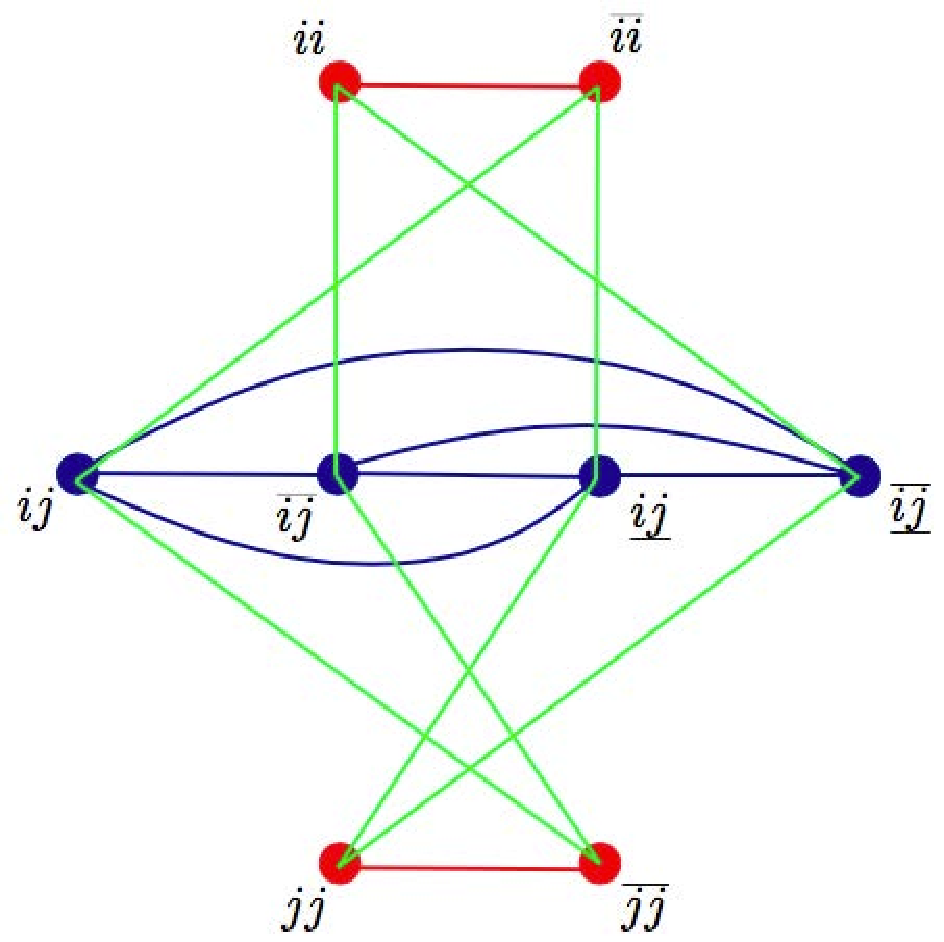
\includegraphics[scale=0.4]{stable.pdf}
\caption{The set of edges and vertices added to $H_n$ for some $i,j \in [n]$ with $i < j$.}
\label{fig:stab-construct}
\end{figure}

Next, we designate the face $F$ of $\STAB(H_n)$ that will be an extension of $\COR(n)$. Note that in the construction, every vertex $i$ in $K_n$ has two vertices associated with it: $ii$ and $\ol{ii}$. These vertices form a clique in $H_n$. We will call these \emph{vertex cliques}. Also, every edge label $ij$ in $K_n$ has four vertices associated with it: $ij, \ol{ij}, \ul{ij}, \oul{ij}$. These vertices form a clique in $H_n$. We will call these \emph{edge cliques}. Then we let $F$ be the face of $\STAB(H_n)$ whose vertices correspond to the stable sets containing exactly one vertex in each vertex-clique and each edge clique. 

Next, we are ready to propose a linear map that will prove that $F$ is in fact an extension of $\COR(n)$. Let $\pi : \R^{V(H_n)} \to \R^{n\times n}$ be defined such that $\pi(x)$ maps to $y \in \R^{n \times n}$ where $y_{ij} = y_{ji} = x_{ij}$ for $i \le j$. We claim that $\pi(F) = \COR(n)$, which would imply that $F$ is an extension of $\COR(n)$.

We start by showing $\pi(F) \subseteq \COR(n)$. Let $\chi^S \in F$. Then let $b \in \bits^n$ such that $b_i = 1$ if $ii \in S$ and $b_i = 0$ if $\ol{ii} \in S$. As $\chi^S \in F$, we have that $S$ contains exactly one vertex from every vertex clique and exactly one vertex from every edge clique. Thus, if $ij \in S$, then $\ol{ii}$ and $\ol{ij}$ cannot be in $S$ since the edges $\{ij, \ol{ii}\}$ and $\{ij, \ol{jj}\}$ are in $H_n$. Then we have that $ii$ and $jj$ must be in $S$. Furthermore, if $ii$ and $jj$ are in $S$, then it must be the case that $ij \in S$. If this were not true, then either $\ol{ij}$, $\ul{ij}$, or $\oul{ij}$ would be in $S$, but all of these have an edge either to $ii$ or $jj$ in $H_n$, so this would contradict the fact that $S$ is a stable set. Therefore, we have that $ij \in S$ if and only if $ii$ and $jj$ are in $S$. Let $x = \chi^S$. Then $x_{ii} = 1$ if and only if $b_{ii} = 1$ by definition of $b_i$. Note that $(bb^T)_{ii} = b_{ii}$. Also, $x_{ij} = 1$ for $i < j$ if and only if $ii$ and $jj$ belong to $S$ as we argued above, which is equivalent to $b_{ii}b_{jj} =1$, by definition of $b$. Note that $(bb^T)_{ij} = (bb^T)_{ji} = b_{ii}b_{jj}$. Thus, we have that $\pi(x) = bb^T$, which is a vertex of $\COR(n)$, by Definition~(\ref{def:cor}). So $\pi(F) \subseteq \COR(n)$.

Finally, we show $\COR(n) \subseteq \pi(F)$. Let $y = bb^T$ be a vertex of $\COR(n)$. We now want to construct an $x = \chi^S \in F$ such that $\pi(x) = y$. So let $S$ be the set that contains vertex $ii$ if $b_i = 1$ and vertex $\ol{ii}$ if $b_i = 0$. By the argument in the preceding paragraph showing $ij \in S$ if and only if $ii$ and $jj$ are both in $S$, it follows that $x$ is a vertex of $F$ such that $\pi(x) = y$. Therefore, $\COR(n) \subseteq \pi(F)$ and we have $\COR(n) = \pi(F)$, which is what we wanted to show.
\end{proof}

The following result is essentially a consequence of Lemma~(\ref{lem:stab-reduct}).

\begin{theorem}\label{thm:stab-reduct}
For all $n$, there exists a graph $G_n$ with $n$ vertices such that $\xc(\STAB(G_n)) = 2^{\Omega(\sqrt{n})}$.
\end{theorem}
\begin{proof}
Recall from the proof of Lemma~(\ref{lem:stab-reduct}) that the size of $H_\ell$ was $2\ell + 4\binom{\ell}{2}$, where the $2\ell$ factor came from the vertex cliques and the $4\binom{\ell}{2}$ came from the edge cliques. Thus, this construction will not work for all $n$ if we use $H_n$. Thus, we proceed as follows. Construct $G_n$ from $H_\ell$ by adding $n - (2\ell + 4\binom{\ell}{2})$ isolated vertices where $\ell$ is the largest integer such that $n - (2\ell + 4\binom{\ell}{2})$ is nonnegative. Then $\STAB(H_\ell)$ is linearly isomorphic to a face of $\STAB(G_n)$ (specifically, the face that contains stable sets with vertices in $H_\ell$). Thus, it easily follows that $\xc(\STAB(G_n)) \ge \xc(\STAB(H_\ell))$ as they are linearly isomorphic.

Then by Lemma~(\ref{lem:stab-reduct}), we know that $\STAB(H_\ell)$ contains a face that is an extension of $\COR(\ell)$, so by part (2) of Lemma~(\ref{lem:reduct}), we have that $\xc(\STAB(H_\ell)) \ge \xc(\COR(\ell))$. From Theorem~(\ref{theor:cut}), we know that $\xc(\COR(\ell)) = 2^{\Omega(\ell)}$. Finally, as $\ell$ is the largest integer such that $n - (2\ell + 4\binom{\ell}{2}) = n - 2\ell^2$, it follows that $n - 2\ell^2 \ge 0$ and $n - 2(\ell + 1)^2 < 0$, which implies $\ell = \Theta(\sqrt{n})$. Therefore, we have $2^{\Omega(\ell)} = 2^{\Omega(\sqrt{n})}$. Combining all of the previous statements in this paragraph, we have $\xc(\STAB(G_n)) = 2^{\Omega(\sqrt{n})}$.
\end{proof}

\subsection{Reduction from $\TSP(n)$}

In this subsection, we will sketch the result of Fiorini~\cetal~\cite{fiorini} showing that the extension complexity of the traveling salesman problem polytope is exponential. This is the main result of \cite{fiorini}, settling the extension complexity of $\TSP(n)$, and extending Yannakakis's result \cite{yannakakis}, by showing that any LP for $\lang{TSP}$, even an asymmetric one, has exponential size. For brevity, we will provide a brief sketch of the proof, as it is quite similar to the reduction presented in Section \ref{sec:stab}.

We first provide a formal definition of $\TSP(n)$.

\begin{definition}[$\TSP$ Polytope]
Let $K_n = (V_n, E_n)$ be the complete graph with $n$ vertices. Recall that a characteristic vector for a set of edges $F \subseteq E_n$ is $\chi^F = \left(\chi^{e_1}, \cdots, \chi^{e_m}\right)$, where $\chi^e = 1$ if $e \in F$ and $\chi^e = 0$ if $e \notin F$, while $m = \frac{n(n-1)}{2}$. The \emph{Traveling Salesman Problem polytope} $\TSP(n)$ is defined as the convex hull of the characteristic vectors of all $F \subseteq E_n$ such that $F$ is a Hamiltonian cycle of $K_n$. In other words,
\[
\TSP(n) \coloneqq \conv\left(\left\{\chi^F \in \R^{E_n} \mid F \subseteq E_n \text{ is a Hamiltonian cycle of $K_n$}\right\}\right).
\]
\end{definition}

Next, we state the main result of this section, as well as of \cite{fiorini}.

\begin{lemma}\label{lem:tsp-reduct}
For every $n$, there exists a positive integer $q = O(n^2)$ such that $\TSP(q)$ contains a face that is an extension of $\COR(n)$.
\end{lemma}
\begin{proofsketch}
First, recall that
\[
\COR(n) \coloneqq \conv\left( \left\{ bb^T \in \R^{n \times n} \mid b \in {\{0, 1\}}^n \right\} \right)
\]
The proof follows the standard reduction of Sipser \cite{sipser} from $\THREESAT$ to $\HAMPATH$ very closely. The authors of \cite{fiorini} show the Lemma using the following steps
\begin{enumerate}
\item They first construct a $\THREESAT$ formula $\phi$ with $n^2$ variables, such that any satisfying assignment of the $n^2$ variables bijectively corresponds to the entries of a matrix $b b^T$, where $b \in {\{0, 1\}}^n$.

\item Next, they create a directed graph $D$ with $O(n^2)$ vertices, such that every Hamiltonian cycle of $D$ surjectively corresponds to a satisfying assignment of $\phi$. Note however that a satisfying assignment of $\phi$ could be obtained by two different Hamiltonian cycles of $D$.

\item In the next step, they create an undirected graph $G$ from $D$ again with $O(n^2)$ vertices, while ensuring that the mapping from satisfying assignments to Hamiltonian cycles is now bijective in $G$. Thus, every Hamiltonian cycle of $G$ bijectively corresponds to a matrix $b b^T$, where $b \in {\{0, 1\}}^n$, and thus to a vertex of $\COR(n)$. Critically, the graph $G$ created at this step is not a clique.

\item Finally, let $l = |V(G)|$, and $\chi^E$ denote the characteristic vector of the of edges of $K_l$. Notice that, for any set of edges $F \subseteq E(G)$, we have that $\chi^F$ has a $0$ entry for all the non-edges in $G$. In other words, the only characteristic vectors that can express the set of edges of $G$ have a $0$ in all the entries corresponding to edges that are not in $G$. Thus, all such characteristic vectors denote a face of $\TSP(l)$. Let us denote this face by $F_G$. Any vertex of $\COR(n)$, and by convexity any point of $\COR(n)$, corresponds to a vertex of $\TSP(l)$ that lies in the face $F_G$. Since $l = O(n^2)$, and $\TSP(l)$ contains a face that is an extension of $\COR(n)$, the Lemma follows.
\end{enumerate}
\end{proofsketch}

The final theorem of this section now follows immediately from Lemmas \ref{lem:tsp-reduct} and \ref{lem:reduct} and Theorem \ref{theor:cut}.

\begin{theorem}
The extension complexity of $\TSP(n)$ is $2^{\Omega\left(\sqrt{n}\right)}$.
\end{theorem}

We note here that using Theorem $6$ of \cite{Yannakakis}, once can get a $2^{\Omega\left(n^{\frac{1}{4}}\right)}$ lower bound for the extension complexity of the $\TSP(n)$ polytope, using Theorem \ref{thm:stab-reduct}, along with the fact that for every $p$-vertex graph $G$, $\STAB(G)$ is the linear projection of a face of $\TSP(n)$, where $n = O(p^2)$. The authors of \cite{fiorini} observe this fact, before strengthening the lower bound of the extension complexity of $\TSP(n)$.

\section{Conclusion}

\bibliographystyle{unsrt}
\bibliography{refs}
\end{document}
